
\documentclass{article}

\usepackage{graphviz}
\usepackage{url}
\usepackage{hyperref}
\usepackage{fullpage}
\usepackage{parskip}
\usepackage{fancyvrb}
\usepackage{amsmath}
\usepackage[section]{placeins}
\usepackage{tikz-timing}

\usepackage{listings}
\lstset{numbers=left,
		basicstyle=\footnotesize,
		captionpos=b,
		xleftmargin=0.3in}

\usepackage[backend=biber,autocite=footnote,
	            bibstyle=authortitle,citestyle=verbose-inote]{biblatex}
\addbibresource{refs.bib}
\setlength\bibitemsep{1em}

\usepackage[xindy,toc,nonumberlist]{glossaries}
\makeglossaries
\renewcommand*{\glspostdescription}{}

\providecommand{\e}[1]{\ensuremath{\times 10^{#1}}}

\VerbatimFootnotes

\raggedright

\begin{document}

% {{{ glossary entries

\newglossaryentry{SPI}
{
	name={SPI},
	description={Serial peripheral interface}.
}

\newglossaryentry{MOSI}
{
	name={MOSI},
	description={(SPI) master out slave in}.
}

\newglossaryentry{MISO}
{
	name={MOSI},
	description={(SPI) master in slave out}.
}

\newglossaryentry{GPIO}
{
	name={GPIO},
	description={General purpose input/output}.
}

\newglossaryentry{FIFO}
{
	name={FIFO},
	description={First in first out}.
}

% }}}

% {{{ title page
\vspace*{1.0in}

\centerline{\LARGE \textbf{SprinklerPI}}
\vspace{0.3in}
\centerline{\LARGE Product Design}

\vfill

\begin{center}
\begin{tabular}{c}
Jeremiah Mahler \\
EECE 490B, CSU Chico \\
May 6, 2014
\end{tabular}
\end{center}

\vspace{2in}

\thispagestyle{empty}

\pagebreak
% }}}

\nocite{rasberrypi}
\thispagestyle{empty}
\tableofcontents

% {{{ Architectural Design
\clearpage
\section{Architectural Design}

SprinklerPI is a web based sprinkler control system.
At the highest level it provides a web interface
which allows watering schedules to be created and modified.
To serve this web interface requires a web server.
In this case a web server running on Linux is used.

Each control/driver module can drive eight sprinkler valves.
And they accepts commands sent over SPI.
They can also be daisy chained together to drive more valves.
Since the RasberryPI can communicate over SPI it also
acts as the master of the SPI bus and sends these commands.

Between the web server and the SPI device both queuing and scheduling
must be performed.
A web server is not suited for these tasks because it is request driven.
To bridge this gap a set of daemons are provided.
Each one handles a specific tasks such as scheduling or queuing.

The communication channel between the web server and the daemons is the
file system.
A specific set of files at specific locations stores the entire state
of the system.
And these files are all in human readable format so they
can be accessed using standard command line tools.

And to power all of these devices requires a power supply capable
of providing both 24 volts AC and 3.3 volts DC.

Figure \ref{fig:spioview} shows an overview of the system.

\begin{figure}[h!]
\begin{center}
\includegraphics[scale=0.40]{dia/sprinklerpi_overview}
\end{center}
\caption{Overview of main components inside the SprinklerPI system.}
\label{fig:spioview}
\end{figure}

\pagebreak
When this system is installed on a private network or behind a firewall
it cannot be accessed from the Internet.  With the addition of a
client/server water daemon, that acts as a proxy, this system can still be
used as shown in Figure \ref{fig:spioviewnet}.

\begin{figure}[h!]
\begin{center}
\includegraphics[scale=0.40]{dia/sprinklerpi_overview-net}
\end{center}
\caption{SprinklerPI system configured for access behind a firewall.}
\label{fig:spioviewnet}
\end{figure}

% }}}

% {{{ Hardware Design
\clearpage
\section{Hardware Design}
\label{sec:hardware}

There are three main hardware components in this system:
the power supply, the Linux computer, and the control/driver.
Figure \ref{fig:hwoview} gives an overview of the hardware in the system.

\begin{figure}[h!]
\begin{center}
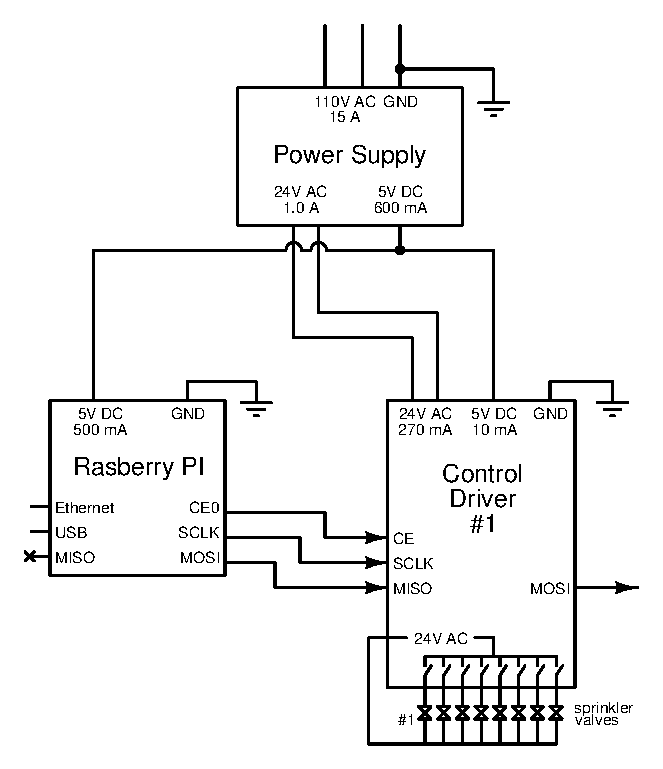
\includegraphics[scale=0.9]{xcircuit/hardware_overview}
\end{center}
\caption{Overview of hardware in system.
Only one control/driver is shown, 
additional control/drivers can be added up to a maximum of three.}
\label{fig:hwoview}
\end{figure}

The power supply takes 24 volts AC and outputs 3.3 volts DC
and 24 volts AC..
The 3.3 volts DC is used by the digital logic and the Linux computer.
The 24 volts AC is used to driver the sprinkler valves.
The power supply also includes an in line fuse to limit the current in
the AC circuit.

The Linux computer is a RasberryPI model B.
It communicates over Ethernet or using a wireless adapter.
And it communicates to the control/driver modules using SPI.

The control/driver accepts commands over SPI to turn on a particular valve.
It then switches the 24 volts AC supply using a triac to turn on a valve.
The control/driver can also be daisy chained to expand it up to a maximum
of three control/drivers.

\pagebreak

% {{{ State Flow Diagrams
\subsection{State Flow Diagrams}

The control/driver goes through two states as shown
in Figure \ref{fig:hwoview}.
When it is not receiving a command it is in the drive state.
In this state it is decoder is enabled and it is either driving
a valve or all valves are off.
In the receive command state the output decoder is disabled to
prevent incorrect intermediate states during transfer.
When it is disabled it will retain its previous value.
When the reception of a command over SPI is complete, the decoder
is re-enabled.

\begin{figure}[h!]
\centering
\includegraphics[scale=0.40]{dia/hardware_state}
\caption{State diagram of control/driver.}\label{fig:hwstate}
\end{figure}

% }}}

% {{{ Schematics
\clearpage
\FloatBarrier
\subsection{Schematics}

% {{{ Control
\FloatBarrier
\subsubsection{Control}
\label{sec:control}

The control part of the control/driver module interprets the commands
received over SPI which determines which valve will be driven or whether
they will be all off.
The driver will be discussed in more detail in Section \ref{sec:driver}.

Typical sprinkler systems can drive valves in groups of eight where only
one valve can be on at a
time\footnote{If multiple circuits were active this could lower the
water pressure resulting in inconsistent watering amounts.}.
This control module achieves this constraint in hardware by using a
decoder chip which only allows one output to be on at a time.

SPI is used to communicate between the Linux computer and the control
module.
Each module uses a 4-bit shift register but a minimum of 8-bits must
be sent per message from the Linux computer.
Additionally, when control/driver modules are daisy chained, more than
8-bits must be sent.

Figure \ref{fig:spi} shows the message format that is used.
Notice that there is a dedicated enable bit and it is active low.
Only 4-bits are used to address the valve.

{
\renewcommand*\arraystretch{1.5}
\begin{figure}[hbp]

\centering

\begin{tabular}{l r l r l r }
7 & 4 & 3 & 1 & \multicolumn{2}{c}{0} \\
\hline
\multicolumn{2}{|c|}{\hspace*{6mm} unused \hspace*{6mm}} &
\multicolumn{2}{|c|}{\hspace*{4mm} valve (group \#1) \hspace*{4mm}} &
\multicolumn{2}{|c|}{\hspace*{1mm} en\_n \hspace*{1mm}} \\
\hline
\end{tabular} \\
(a)

\begin{tabular}{l r l r l r l r }
7 & 5 & \multicolumn{2}{c}{4} & 3 & 1 & \multicolumn{2}{c}{0} \\
\hline
%\multicolumn{2}{|c|}{\hspace*{6mm} unused \hspace*{6mm}} &
\multicolumn{2}{|c|}{\hspace*{4mm} valve (group \#2) \hspace*{4mm}} &
\multicolumn{2}{|c|}{\hspace*{1mm} en\_n \hspace*{1mm}} &
\multicolumn{2}{|c|}{\hspace*{4mm} valve (group \#1) \hspace*{4mm}} &
\multicolumn{2}{|c|}{\hspace*{1mm} en\_n \hspace*{1mm}} \\
\hline
\end{tabular} \\
(b)

\caption{SPI message format for one group (a) and two groups (b).
Each group represents eight valves so (b) would support 16 valves.}
\label{fig:spi}
\end{figure}
}

Interpreting the message received is performed using a shift register
and decoder as shown in Figure \ref{fig:control}.
An output high of the decoder will turn on a valve.
Notice that the enable bit in the message will be output on \verb+OA+
which will enable the decoder chip.

\begin{figure}[hbp]
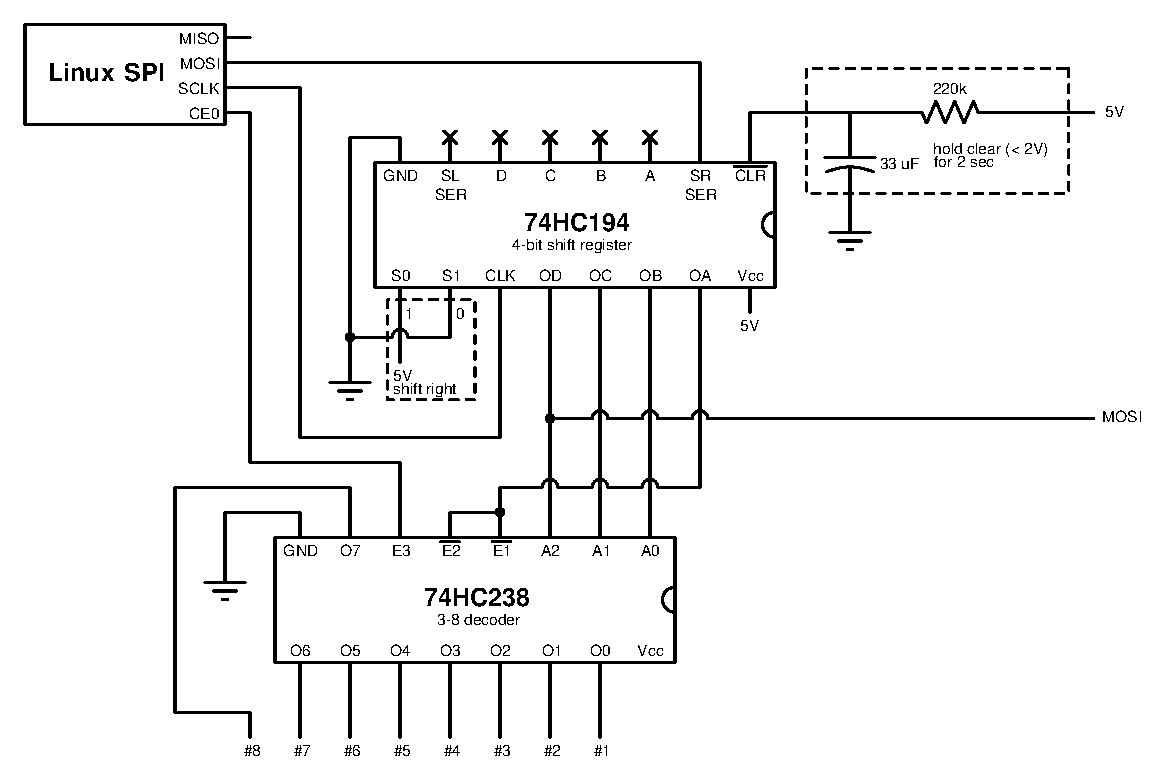
\includegraphics[scale=0.85]{xcircuit/control}
\caption{Sprinkler valve control logic.
Sprinkler valve number is input using SPI from the Linux computer in
to the shift register.
A 4-bit number is output from the shift register and sent to the
decoder which will turn on a valve or turn them all off.
All outputs are disabled when OA is clear.}\label{fig:control}
\end{figure}

% }}}

% {{{ Expansion
\clearpage
\subsubsection{Expansion}
\label{sec:expansion}

Each control/driver module accepts a command over SPI.
And depending on the message it receives it will turn one of the
eight valves on or turn them all off.
And up to three of these modules can be daisy chained together
to expand the system to a maximum of 24 valves.
This daisy chain configuration is shown in Figure \ref{fig:expansion_spi}.

\begin{figure}[hbp]
\centering
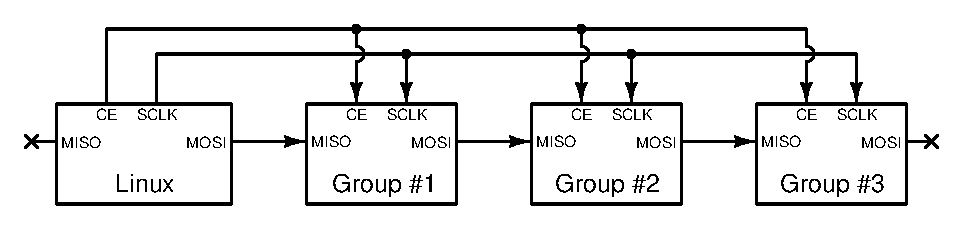
\includegraphics[angle=0,scale=0.80]{xcircuit/expansion_spi}
\caption{Daisy chain SPI configuration for multiple control groups.
}\label{fig:expansion_spi}
\end{figure}

The power supply is the limiting factor in expansion beyond three
modules as shown in Figure \ref{fig:expansion_current}.

\begin{figure}[hbp]
\centering
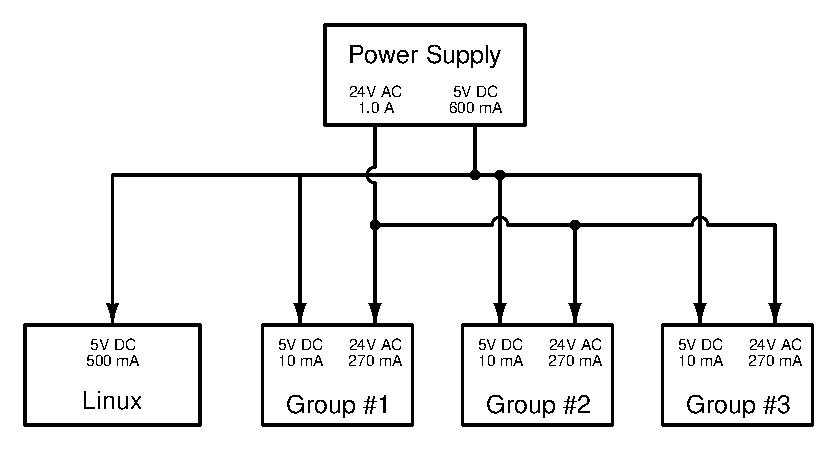
\includegraphics[angle=0,scale=0.80]{xcircuit/expansion_current}
\caption{With a power supply capable of 1 amp at 24 volts AC and
600 mA at 3.3 volts DC a maximum of three control groups and one
Linux computer can be driven.}\label{fig:expansion_current}
\end{figure}

% }}}

\pagebreak

% {{{ Driver
\FloatBarrier
\subsubsection{Driver}
\label{sec:driver}

The control part of the control/driver module (Section \ref{sec:control})
determines which valve will be driven.  But it cannot drive the valves
directly as they require 24 volts AC and the control circuit outputs
3.3 volts DC.
The purpose of the driver part of the control/driver module is to convert
these digital signal and drive the valves.
The driver circuitry is shown in Figure \ref{fig:driver}.

\begin{figure}[hbp]
\centering
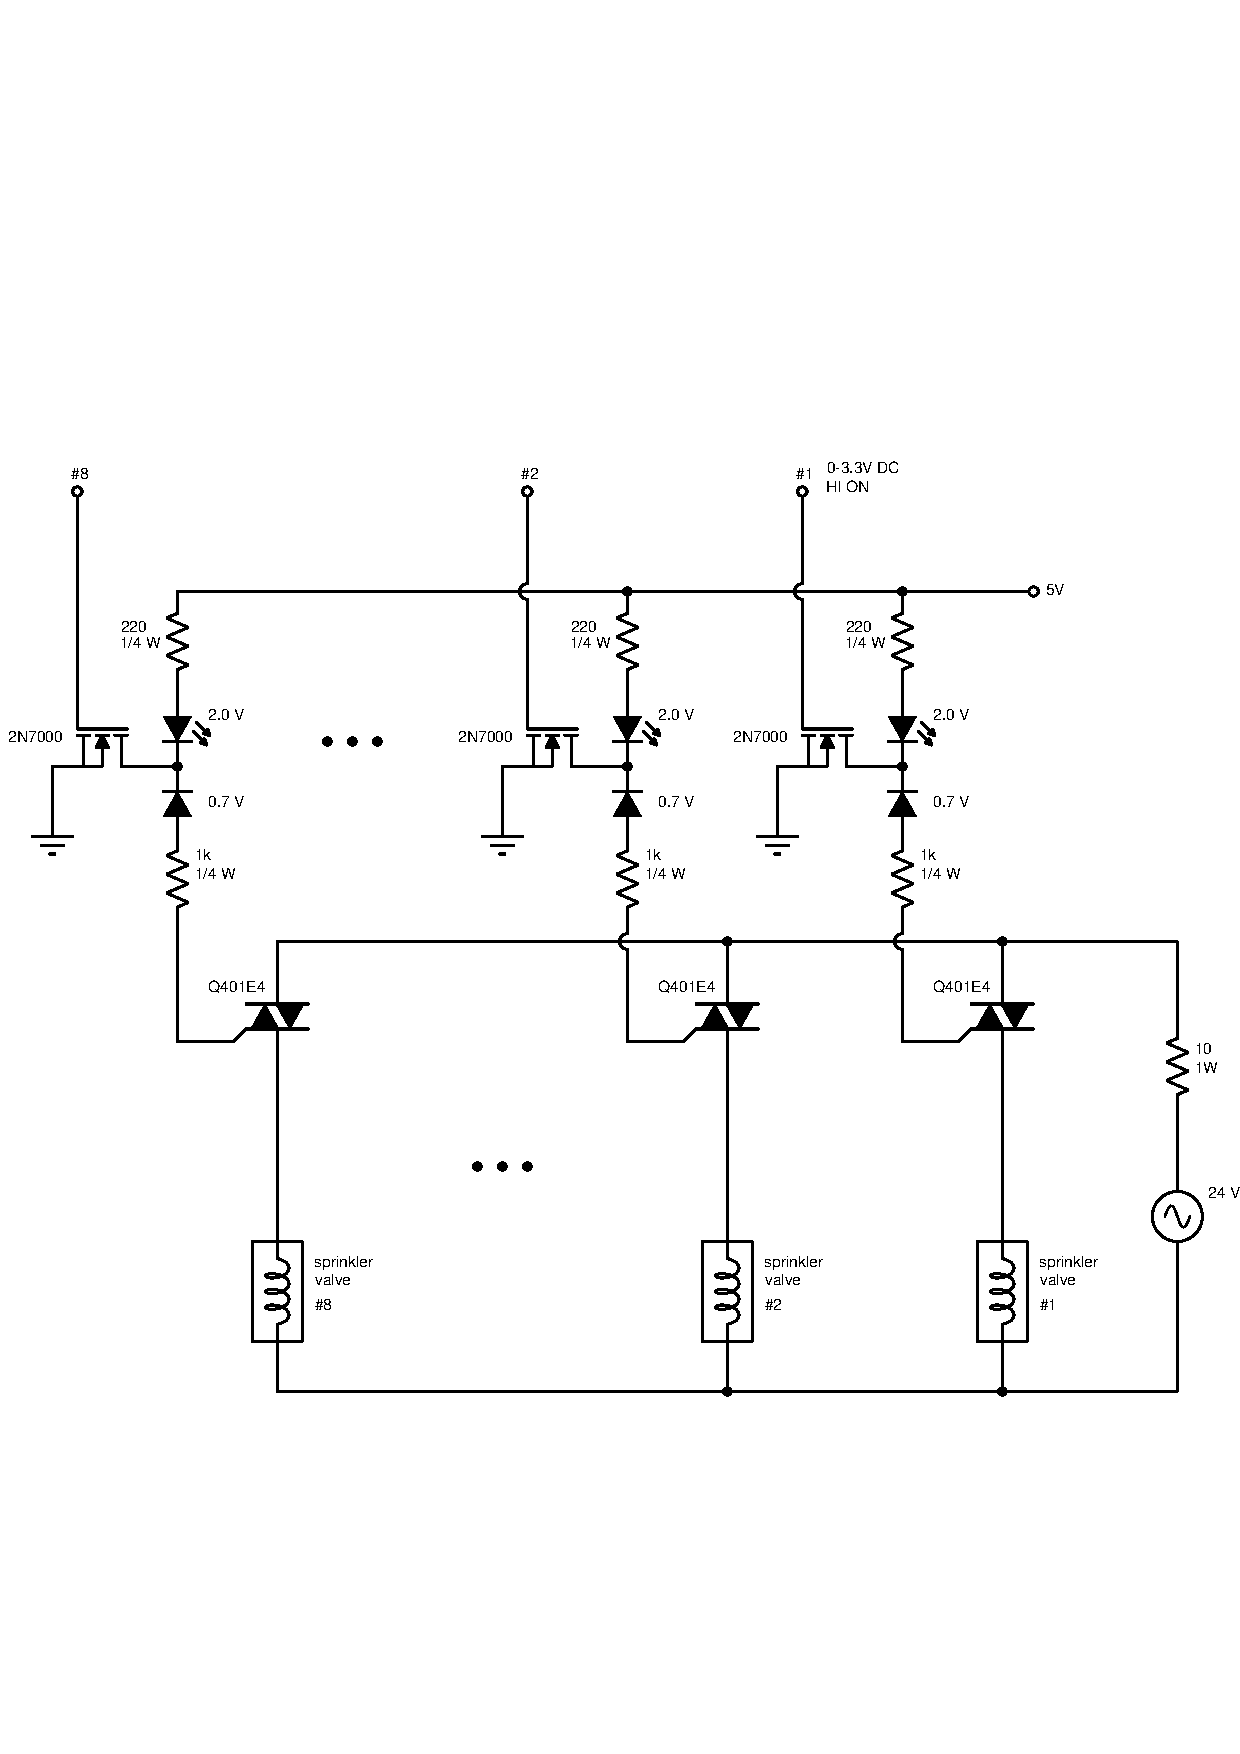
\includegraphics[scale=0.7]{xcircuit/driver_mult}
\caption{Sprinkler valve driver circuits.
Not all branches are shown since they are identical.
LEDs are used to indicate when the valve is on/off.
It is assumed that only one valve will be on at a time.}\label{fig:driver}
\end{figure}

To turn the sprinkler valves on requires 24 volts AC at approximately 270 mA.
Each sprinkler valve has a resistance of approximately 80 $\Omega$.
A 10 $\Omega$ resistor was added to limit the current to 270 mA.
A resistor with a 1 watt rating provides over a 10\% operating margin.

\begin{align*}
	P &= I^2 R \\
	  &= (270\e{-3})^2 \cdot 10 \\
	  &= 0.729 \quad \text{[W]}
\end{align*}

The control signal to the triac (Q401E4) is very sensitive.
The tiniest of currents in either direction will turn it on.
A diode is used to restrict the current to one direction and ensure
that the triac will switch off.
The FET (2N7000) drives the triac as well as the LED indicator.
It also serves to limit the gate current required from the control module.
The required gate current is less than 0.5 mA which is well within
the limits of CMOS logic used by the control module (Section \ref{sec:control}).

% }}}

% {{{ Power Supply
\subsubsection{Power Supply}
\label{sec:power}

The power supply must provide two different voltages: 24 volts AC and
3.3 volts DC.
The sprinkler valves require 24 volts AC at 270 mA.
The Linux computer and other digital logic require 3.3 volts DC with a
maximum draw of 600 mA
\footnote{The current draw of the RasberryPI was determined
experimentally to be approximately 500 mA.}.
These voltages must be created from a 24 volt AC input.
The 24 volts AC is converted from 110 volts AC using a transformer.
Plug mounted 110 to 24 volts AC transformers are commonly available
as most sprinkler controllers use these.

A switching voltage regulator, the MC34063A, was chosen for
the 3.3 volt supply.
It has a greater efficiency than a linear regulator such as
the LM7805.

The circuit which achieves all of these design requirements is
shown in Figure \ref{fig:power}.

\begin{figure}[hbp]
\centering
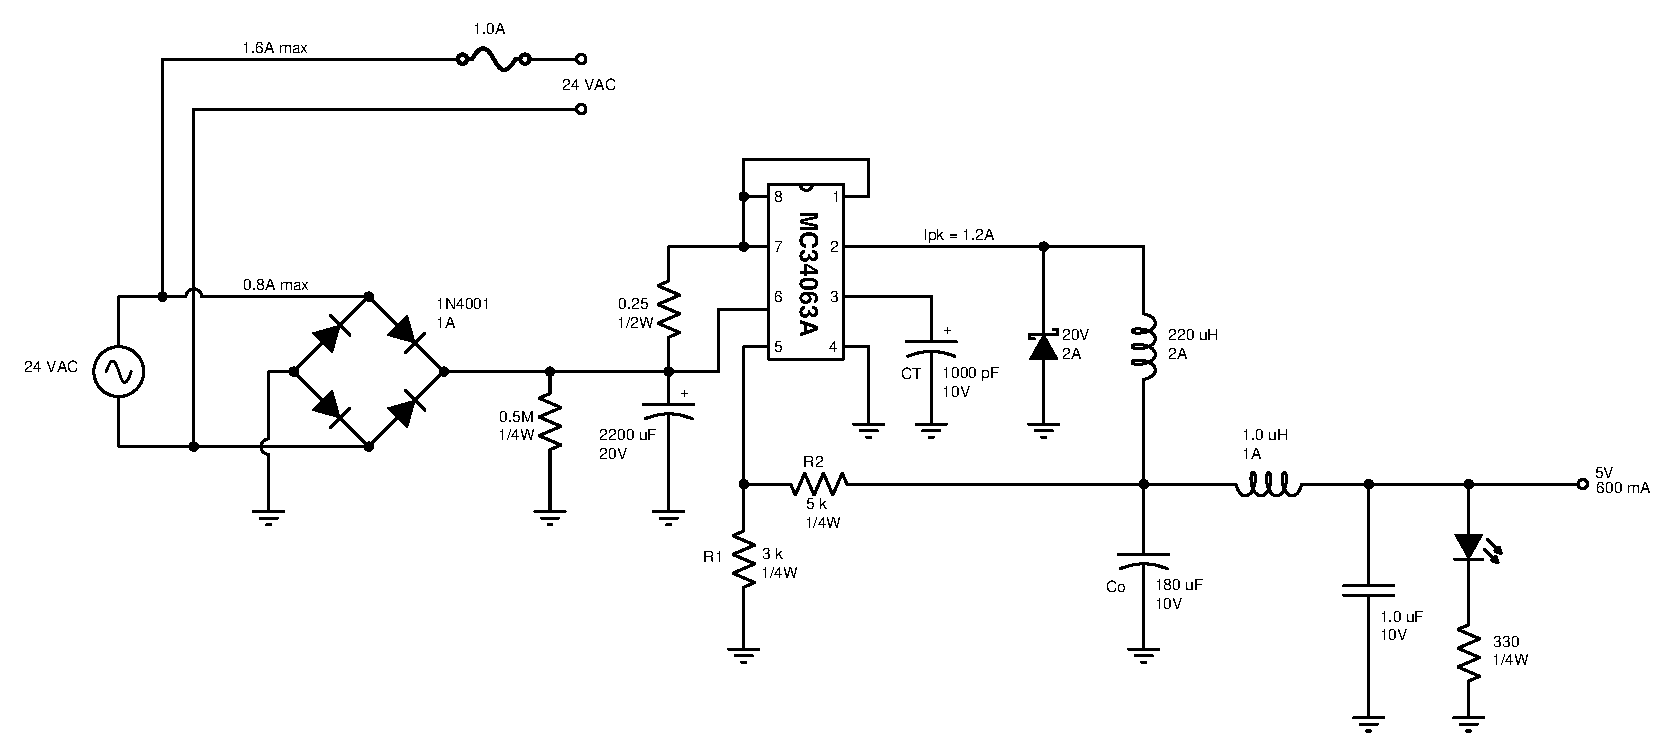
\includegraphics[angle=90,scale=0.70]{xcircuit/power_supply}
\caption{Power supply circuit. A 24 volt AC and 3.3 volt DC output are
provided.  The 3.3 volt DC is provided by the MC340363A switching
regulator.}\label{fig:power}
\end{figure}

% }}}

% }}}

% {{{ Timing Diagrams
\FloatBarrier
\subsection{Timing Diagrams}

Figure \ref{fig:timing} is a diagram of a message being sent
using SPI from the Linux computer to the control module.
Refer to Section \ref{sec:control} for a description of
the meaning of these messages.

\begin{figure}[h!]
\begin{center}
\begin{tikztimingtable}
	[xscale=2.0, yscale=2.0]
	CE	 & {1H} 1{C} {12L} 1{C} {1H} \\
	SCLK & {1H} 14{C} {1H} \\
	MOSI & 10L 1{C} 1{H} 1{C} 3L \\
	MISO & 16L \\
\end{tikztimingtable}
\end{center}
\caption{Timing diagram of a message sent using SPI from
the RasberryPI to a control module.
A value from MOSI is latched on the rising edge of SCLK.
In this case the value 2 is transferred.}
\label{fig:timing}
\end{figure}
% }}}

% {{{ Theory of Operation
%\FloatBarrier
%\subsection{Theory of Operation}
%
%% describe external interface
%
%The operation of the hardware as a whole provides the ability to
%turn a valve on or to turn them all off.
%One valve can be on at a time for a single Control Driver module.
%Commands are written over SPI from the Linux computer (RasberryPI).
%
%The user interface, described in Section \ref{sec:swdesign}, will
%establish a friendly user interface on top of this simple hardware
%interface.

% }}}

% }}}

\pagebreak

% {{{ Software Design
\FloatBarrier
\section{Software Design}
\label{sec:swdesign}

The software in this system consists of many modular parts as
can be seen in Figure \ref{fig:spioview} and Figure \ref{fig:spioviewnet}.

There are several daemons and a web server which all communicate with
each other using the file system as shown in Figure \ref{fig:dov}.
These files can even be edited using command line tools and
they are all stored in a human readable format.
The daemons use the Linux inotify interface so they can receive
file change events without having to poll files.

\begin{figure}
\begin{center}
\includegraphics[scale=0.40]{dia/daemon_oview}
\end{center}
\caption{Overview daemons and how they interact with the web interface
and file system.}
\label{fig:dov}
\end{figure}

The web interface is written using html, PHP, style sheets (CSS), JavaScript,
and can run on any standard web server such as Apache or Nginx.
It provides an interface where schedules can be managed and valves can
be operated.

Each of the daemons has one specific task.
The queue daemon watches the queue and makes sure valves are run
for the correct duration.
The scheduler waits until a valve is scheduled to run and then adds it
to the queue.
The water daemon monitors which valves should be turned on and executes
the command.
There are versions for a local device or a network proxy.

% {{{ File System
\FloatBarrier
\subsection{File System}

The central communication mechanism for interprocess communication
is the file system.  The daemons, web server, and command line programs
all interact using these specific files.
The file hierarchy is shown in Figure \ref{fig:fs}.

\begin{figure}[h!]

\begin{center}
\begin{minipage}{3in}
\begin{verbatim}
sprinklerpi/
  mode
  valves/
    group-1
    group-2
    group-3
  queue/
    group-1
    group-2
    group-3
  schedules/
    test1.yml
    ...
\end{verbatim}
\end{minipage}
\end{center}
\caption{File system hierarchy of sprinklerpi files.}
\label{fig:fs}
\end{figure}

The \verb+mode+ file contains a string specifying the mode.
The daemons can use this file and only perform their operations while
in a specific mode.
For example the scheduler daemon only operates when in the schedule mode.
If the system is in the manual mode it pauses its operation.

The \verb+valves/group-*+ files each indicate which valve should be
operating for that group.
It contains a number, in ascii format, from 0 to 8.
When it is set to zero the valve is off.
The water daemon monitors the valve files and executes the water command
when they change.

The \verb+queue/group-*+ files each store a queue of jobs waiting to be
executed.
The scheduler daemon will add jobs to the queue and the queue daemon
will remove them.
Entries are removed from the start of the file and added by appending to
the file.
File locking must be used to avoid inconsistent intermediate file states.
The format of a queue file is a line with the valve number and run
time in seconds.  An example is shown in Figure \ref{fig:qf}.

\begin{figure}
\begin{center}
\begin{minipage}{2in}
\begin{verbatim}
1 60
1 900
2 15
\end{verbatim}
\end{minipage}
\end{center}
\caption{An example queue file.}
\label{fig:qf}
\end{figure}

The \verb+schedule/*+ files each store an object that describes a full
schedule.
They are stored using the YAML file format which is human readable
and supported across many programming languages.

\begin{figure}
\begin{center}
\begin{minipage}{3in}
\begin{verbatim}
---
id: test1.yml
name: 'Schedule Test #1'
enabled: 1
entries:
- group: "1"
  valve: "1"
  days: MTWThFSSu
  start_time: 00:50
  run_time: 00:30
- group: "1"
  valve: "2"
  days: MTWThFSSu
  start_time: 00:50
  run_time: 00:30
- group: "1"
  valve: "3"
  days: MWF
  start_time: 00:50
  run_time: 00:30
...
\end{verbatim}
\end{minipage}
\end{center}
\caption{An example schedule file in YAML format.}
\label{fig:sched}
\end{figure}
% }}}

% {{{ Queue Daemon
\FloatBarrier
\subsection{Queue Daemon}
\label{sec:queue}

When in \verb+schedule+ mode, the queue daemon will monitor the queue
and run any jobs that are present.
It monitors all the files for each of the groups.
Each instruction is one line with the valve to run and its duration
in seconds (Figure \ref{fig:qf}).
Figure \ref{fig:queue-daemon} gives a flow chart of its operation.

\begin{figure}[htbp!]
\begin{center}
\includegraphics[scale=0.35]{dia/queue-daemon}
\end{center}
\caption{Flow chart of the queue daemon operation.}
\label{fig:queue-daemon}
\end{figure}

% }}}

% {{{ Scheduler Daemon
\clearpage
\FloatBarrier
\subsection{Scheduler Daemon}

The scheduler daemon waits until jobs in the schedules
become due and then it adds them to the queue.
The format is the same as described for the queue
daemon (Section \ref{sec:queue}).
Figure \ref{fig:scheduler-daemon} gives a flowchart of its operation.

\begin{figure}[htbp!]
\begin{center}
\includegraphics[scale=0.35]{dia/scheduler-daemon}
\end{center}
\caption{Flow chart of the scheduler daemon operation.}
\label{fig:scheduler-daemon}
\end{figure}
% }}}

% }}}

\pagebreak
\glsaddall
\printglossaries

% References
\clearpage
\printbibliography[heading=bibintoc]

\end{document}
